\documentclass[12pt]{article}
\usepackage[shortlabels]{enumitem}
\usepackage{float}
\usepackage{xcolor}
\usepackage[a4paper, top=0.6cm, bottom=0.6cm, left=1.5cm, right=1.5cm]{geometry}
\usepackage{parskip}
\usepackage{setspace}
\usepackage{lmodern}
\usepackage[T1]{fontenc}
\usepackage[brazil]{babel}
\usepackage{hyperref}
\usepackage{graphicx}
\usepackage{amsmath}
\usepackage{amssymb}
\usepackage{amsfonts}
\usepackage{dsfont}

% --- Ajuste fino do título ---
\makeatletter
\renewcommand{\maketitle}{
  \begin{center}
    {\small\bfseries \@title \par}
  \end{center}
  \vspace{-0.1cm} % diminui o espaço entre título e texto
}
\makeatother

\title{Questões Extra - Estatística para Administração - 2025.2}
\date{}

\begin{document}
\maketitle

% Questão para alunos com maiores notas

Um dos programas de TV mais populares na década de 1970 nos Estados Unidos era o programa \textit{Let's Make a Deal}. Nesse programa, 
um participante era convidado a participar de um jogo que funcionava da seguinte forma:

\begin{enumerate}
    \item O jogo conta com um único participante e três portas. 
    \begin{figure}[H]
        \centering
        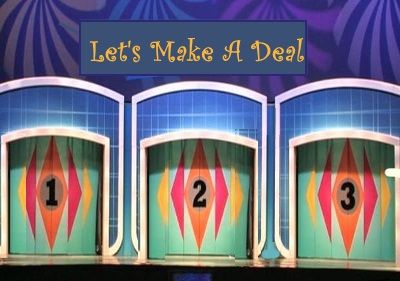
\includegraphics[width=0.5\linewidth]{figures/monty_hall_1.jpeg}
    \end{figure}
    \item Atrás de uma das portas existe um grande prêmio (geralmente um carro), enquanto nas demais temos um prêmio de baixo valor ou absolutamente nada. Ao longo 
    das próximas explicações iremos nos referir a esse prêmio como prêmio ruim. 
    \item O participante deve inicialmente escolher uma das portas. 
    \item O apresentador do programa abre uma porta que não foi escolhida pelo participante, revelando sempre um prêmio ruim.
    \item Após revelar essa porta, restam apenas duas portas, uma é a que a pessoa escolheu inicialmente e a outra é a que restou.
    \item O apresentador então pergunta para o participante se ele deseja trocar ou não a porta escolhida inicialmente. 
    \item Após tomar a decisão, o apresentador abre a porta escolhida.  
\end{enumerate}

Esse programa foi trazido para o Brasil no final da década de 1980 com o nome Porta dos Desesperados, apresentado pelo Sérgio Mallandro. A dinâmica de funcionamento era
a mesma, atrás de uma das portas tinha um grande prêmio, mas atrás das outras portas havia um macaco ou uma múmia. Você pode encontrar alguns episódios tanto do 
programa \textit{Let's Make a Deal} quanto do Porta dos Desesperados no Youtube. 

Dado esse contexto, responda a seguinte pergunta:

Você participa desse programa, o grande prêmio é um carro no valor de R\$ 300.000,00. Você escolhe a porta de número $2$. O apresentador do programa abre a porta de número $1$ revelando que atrás 
dessa porta não tinha nada, restando apenas a porta $2$ (sua escolha inicial) e a porta $3$. O apresentador pergunta se você deseja 
mudar para a porta $3$. 

\begin{enumerate}[a)]
    \item Considere que você está no exato momento de responder ao apresentador se decide trocar ou não a porta escolhida. Qual a probabilidade do prêmio estar na porta $3$?
    Ou seja, dado que o apresentador abriu a porta $1$, qual a probabilidade do grande prêmio estar na porta $3$? E na porta $2$? Use o conceito de probabilidade condicional para resolver 
    essa questão (Lembre-se de definir os eventos relevantes). 
    \item Escreva um pequeno texto discutindo o resultado encontrado anteriormente. Você achou o resultado encontrado surpreendente? Qual indicação você daria para uma pessoa que participa desse programa no momento de decidir se troca ou não de porta?
\end{enumerate}


% Questão para alunos de menores notas. 


% 1)\noindent
% Considere o experimento do lançamento de três dados honestos. 

% \begin{enumerate}[a)]
%   \item Defina um espaço amostral para o experimento e determine sua cardinalidade. 
%   \item Dado que os dois primeiros dados apresentaram  faces com números iguais, qual é a probabilidade da soma dos três dados ser igual a 15?
%   \item Se os dados não fossem honestos, que problema teríamos ao adotar a interpretação clássica da Probabilidade para resolver esse problema?
% \end{enumerate}

% \vspace{0.3cm}

% 2) \noindent
% A empresa Barbelo tem 15.800 empregados, classificados de acordo com a tabela abaixo.

% \begin{center}
% \begin{tabular}{lccc}
% \toprule
% \textbf{Idade (anos)} & \textbf{Homens (M)} & \textbf{Mulheres (F)} & \textbf{Total} \\
% \midrule
% $ (17, 25]$  (A) & 2.000 & 800 & 2.800 \\
%   $(25, 40]$  (B) & 4.500 & 2.500 & 7.000 \\
% $(40, 70]$ (C) & 1.800 & 4.200 & 6.000 \\
% \midrule
% \textbf{Total} & 8.300 & 7.500 & 15.800 \\
% \bottomrule
% \end{tabular}
% \end{center}

% \noindent
% Se um empregado é selecionado ao acaso, calcule a probabilidade dele ser:

% \begin{enumerate}[label=(\alph*)]
%     \item um empregado com 40 anos de idade ou menos;
%     \item um empregado com 40 anos de idade ou menos, e mulher;
%     \item um empregado com mais de 40 anos de idade e que seja homem;
%     \item uma mulher, dado que é um empregado com 25 anos ou menos.
% \end{enumerate}

% \vspace{0.3cm}

% 3)\noindent
% Um teste rápido de triagem para uma determinada doença possui três possíveis resultados: positivo, negativo e incerto. Suponha que ele apresente as seguintes porcentagens:

% \begin{itemize}
%     \item Para uma pessoa com a doença: positivo em 70\% dos casos, negativo em 10\% e incerto em 20\%.
%     \item Para uma pessoa sem a doença: positivo em 10\% dos casos, negativo em 60\% e incerto em 30\%.
% \end{itemize}

% \noindent
% Admita, ainda, que a prevalência da doença na população é de 2\%.

% \medskip

% \noindent
% Qual é a probabilidade de que uma pessoa escolhida aleatoriamente, que testou positivo, realmente tenha a doença? Interprete o valor encontrado. 
% Qual interpretação da Probabilidade foi usada  nessa questão?



\end{document}